\documentclass{beamer}
\usepackage[style=authoryear,urldate=long,backend=biber,natbib=true]{biblatex}
\usepackage{booktabs}
\bibliography{references} 


\usetheme[sectionpage=simple,numbering=fraction,progressbar=frametitle]{metropolis}           % Use metropolis theme
\title{The Himalayan Tightrope}
\subtitle{Balancing the Economy-Environment Trade-off}
\date{Madras School of Economics}
\author{Ritwiz Sarma and Riju Garg}
\institute{59th Annual Conference of the Indian Econometric Society,\\Banaras Hindu University, Varanasi UP\\March 4, 2025}
\begin{document}
    \maketitle
    \begin{frame}{The Trade-off Exists\ldots} % perhaps two onlyenvs, infra side (graphs) vs sustainability side (articles)
        \begin{onlyenv}<1>
        \begin{columns}
        \begin{column}{.45\textwidth}
        \begin{itemize}
            \item Why build infrastructure?
            \begin{itemize}
                \item Network effects, economic growth
                \item Administrative, defense reasons
                \item Political incentives
            \end{itemize}
            % more stuff here
        \vspace*{4.5em}
        \end{itemize}
        \end{column}
        \begin{column}{.45\textwidth}
            \begin{figure}[h]
                \centering
                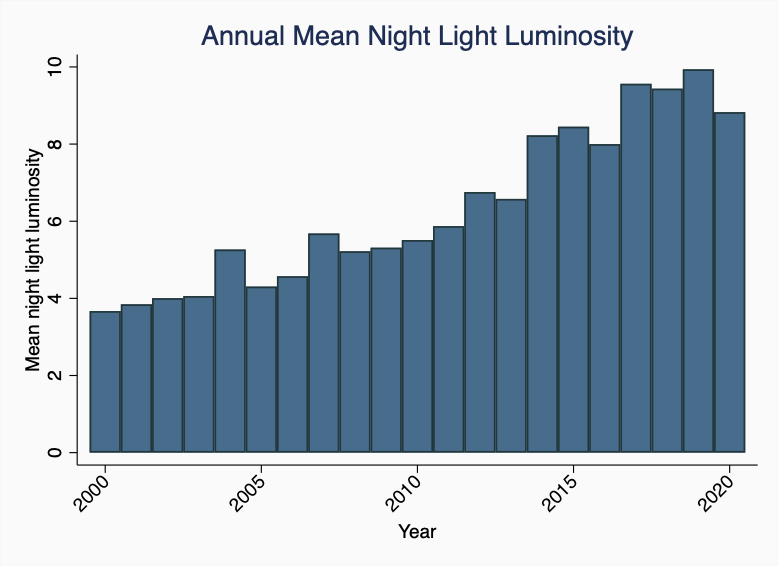
\includegraphics[width=\textwidth]{images/presentation/ntl_trend.png}
                \vspace{2mm}
                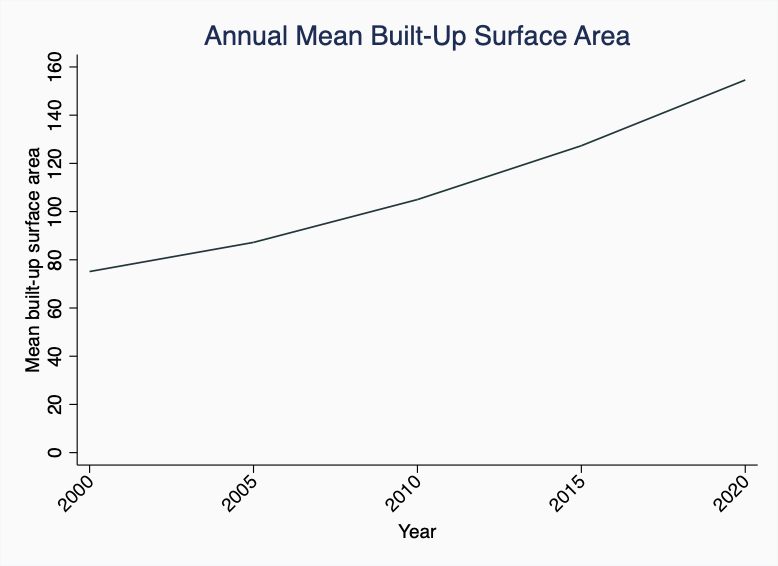
\includegraphics[width=\textwidth]{images/presentation/ghsl_trend.png}
            \end{figure}
        \end{column}
        \end{columns}
        \end{onlyenv}
        \begin{onlyenv}<2>
        \begin{columns}
        \begin{column}{.45\textwidth}
        \begin{itemize}
            \item Why build infrastructure?
            \begin{itemize}
                \item Network effects, economic growth
                \item Administrative, defense reasons
                \item Political incentives
            \end{itemize}
            \item But there is a growing \textit{long-run} and \textit{human} cost.
        \end{itemize}
        \end{column}
        \begin{column}{.45\textwidth}
            \begin{figure}[h]
                \centering
                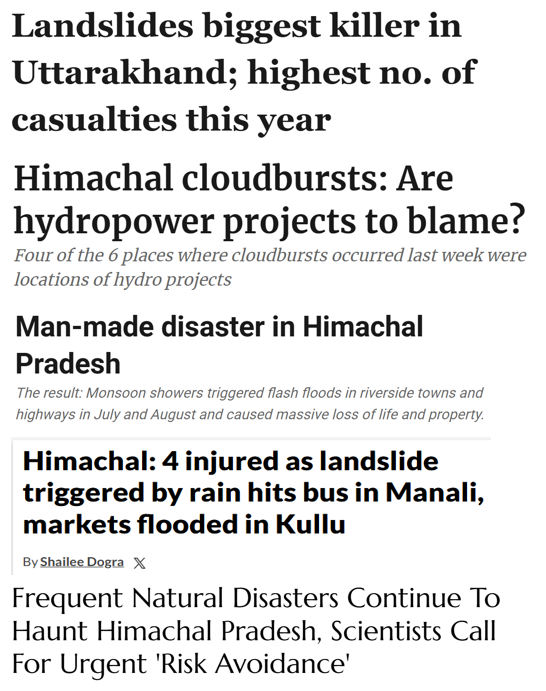
\includegraphics[width=\textwidth]{images/presentation/env_news.png}
            \end{figure}
        \end{column}
        \end{columns}
        \end{onlyenv}
        
    \end{frame}
%fix this
    \begin{frame}{\ldots{}But Do We Measure It Right?} %i feel the need, the need to read
        \begin{columns}
        \begin{column}{.45\textwidth}
        \textbf{Environmental Kuznets Curve}
        \begin{itemize}
            \item Inverted-U relationship between economic growth and environmental degradation.
            \item Contradictory findings in recent literature.
        \end{itemize}
        \end{column}
        \begin{column}{.45\textwidth}
            \begin{figure}[h]
                \centering
                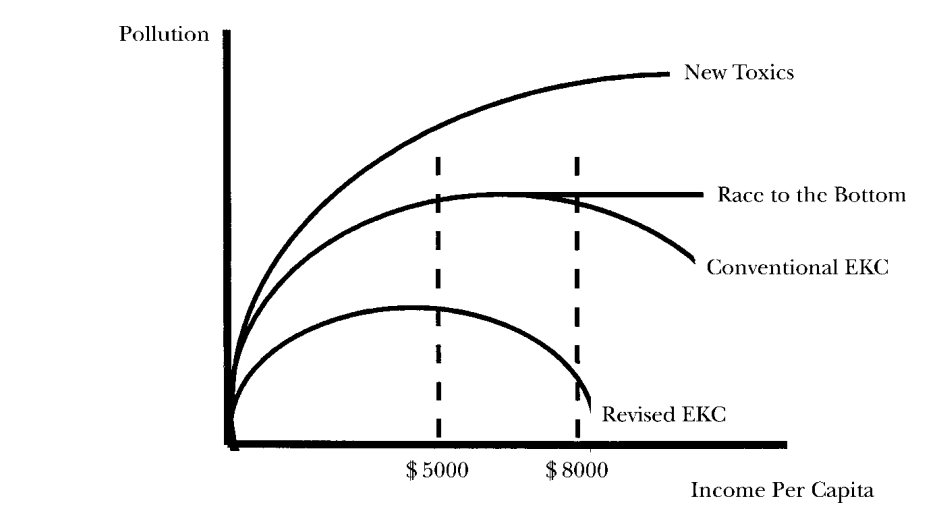
\includegraphics[width=1.1\textwidth]{images/kuznets_scen.png}
                % \vspace{1mm}
                \begin{center}
                    \scriptsize Different EKC adaptations from \textcite{dasgupta2002}.
                \end{center}
                % \caption{Different EKC adaptations from \textcite{dasgupta2002}.}
            \end{figure}
        \end{column}
        \end{columns}
    \end{frame}

    \begin{frame}{Questions}
        \begin{itemize}
            \item How does \textit{infrastructure-led} growth relate to environmental degradation?
            \item Does the Environmental Kuznets curve hold (at the subnational level)?
            \item Do macro-level models hold for: 
            \begin{itemize} % maybe enumerate?
                \item sensitive ecologies?
                \item micro-level data?
            \end{itemize}
        \end{itemize}
    \end{frame}

    \begin{frame}{This Paper}
        Our answer: Not well.\\[2em]

        \begin{itemize}
            % \item We select five indicators for growth and sustainability
            \item We build a high-res geospatial dataset at village/town level
            \item We estimate the EKC: 5 indicators, 20 years of data
            \item We focus on two Himalayan states, where incentives exist for both infrastructure investment and ecological sustainability 
        \end{itemize}
    \end{frame}

    \section{Data}
    \begin{frame}{Dataset Construction}
        \begin{onlyenv}<1>
        \begin{description}
            \item[Shrid] Our base unit of analysis. SHRUG-DevDataLab.\\Usually single village/town, can be aggregation if merged/separated between 1990-2013.
            \item[Indicators] Satellite-based data on infrastructure growth and environmental degradation.
            \item[Indices] Standardization, then take the:
            \begin{itemize}
                \item arithmetic mean, or
                \item principal component 
            \end{itemize}
        \end{description}
        \end{onlyenv}
        \begin{onlyenv}<2>
            \begin{figure}[h]
                \centering
                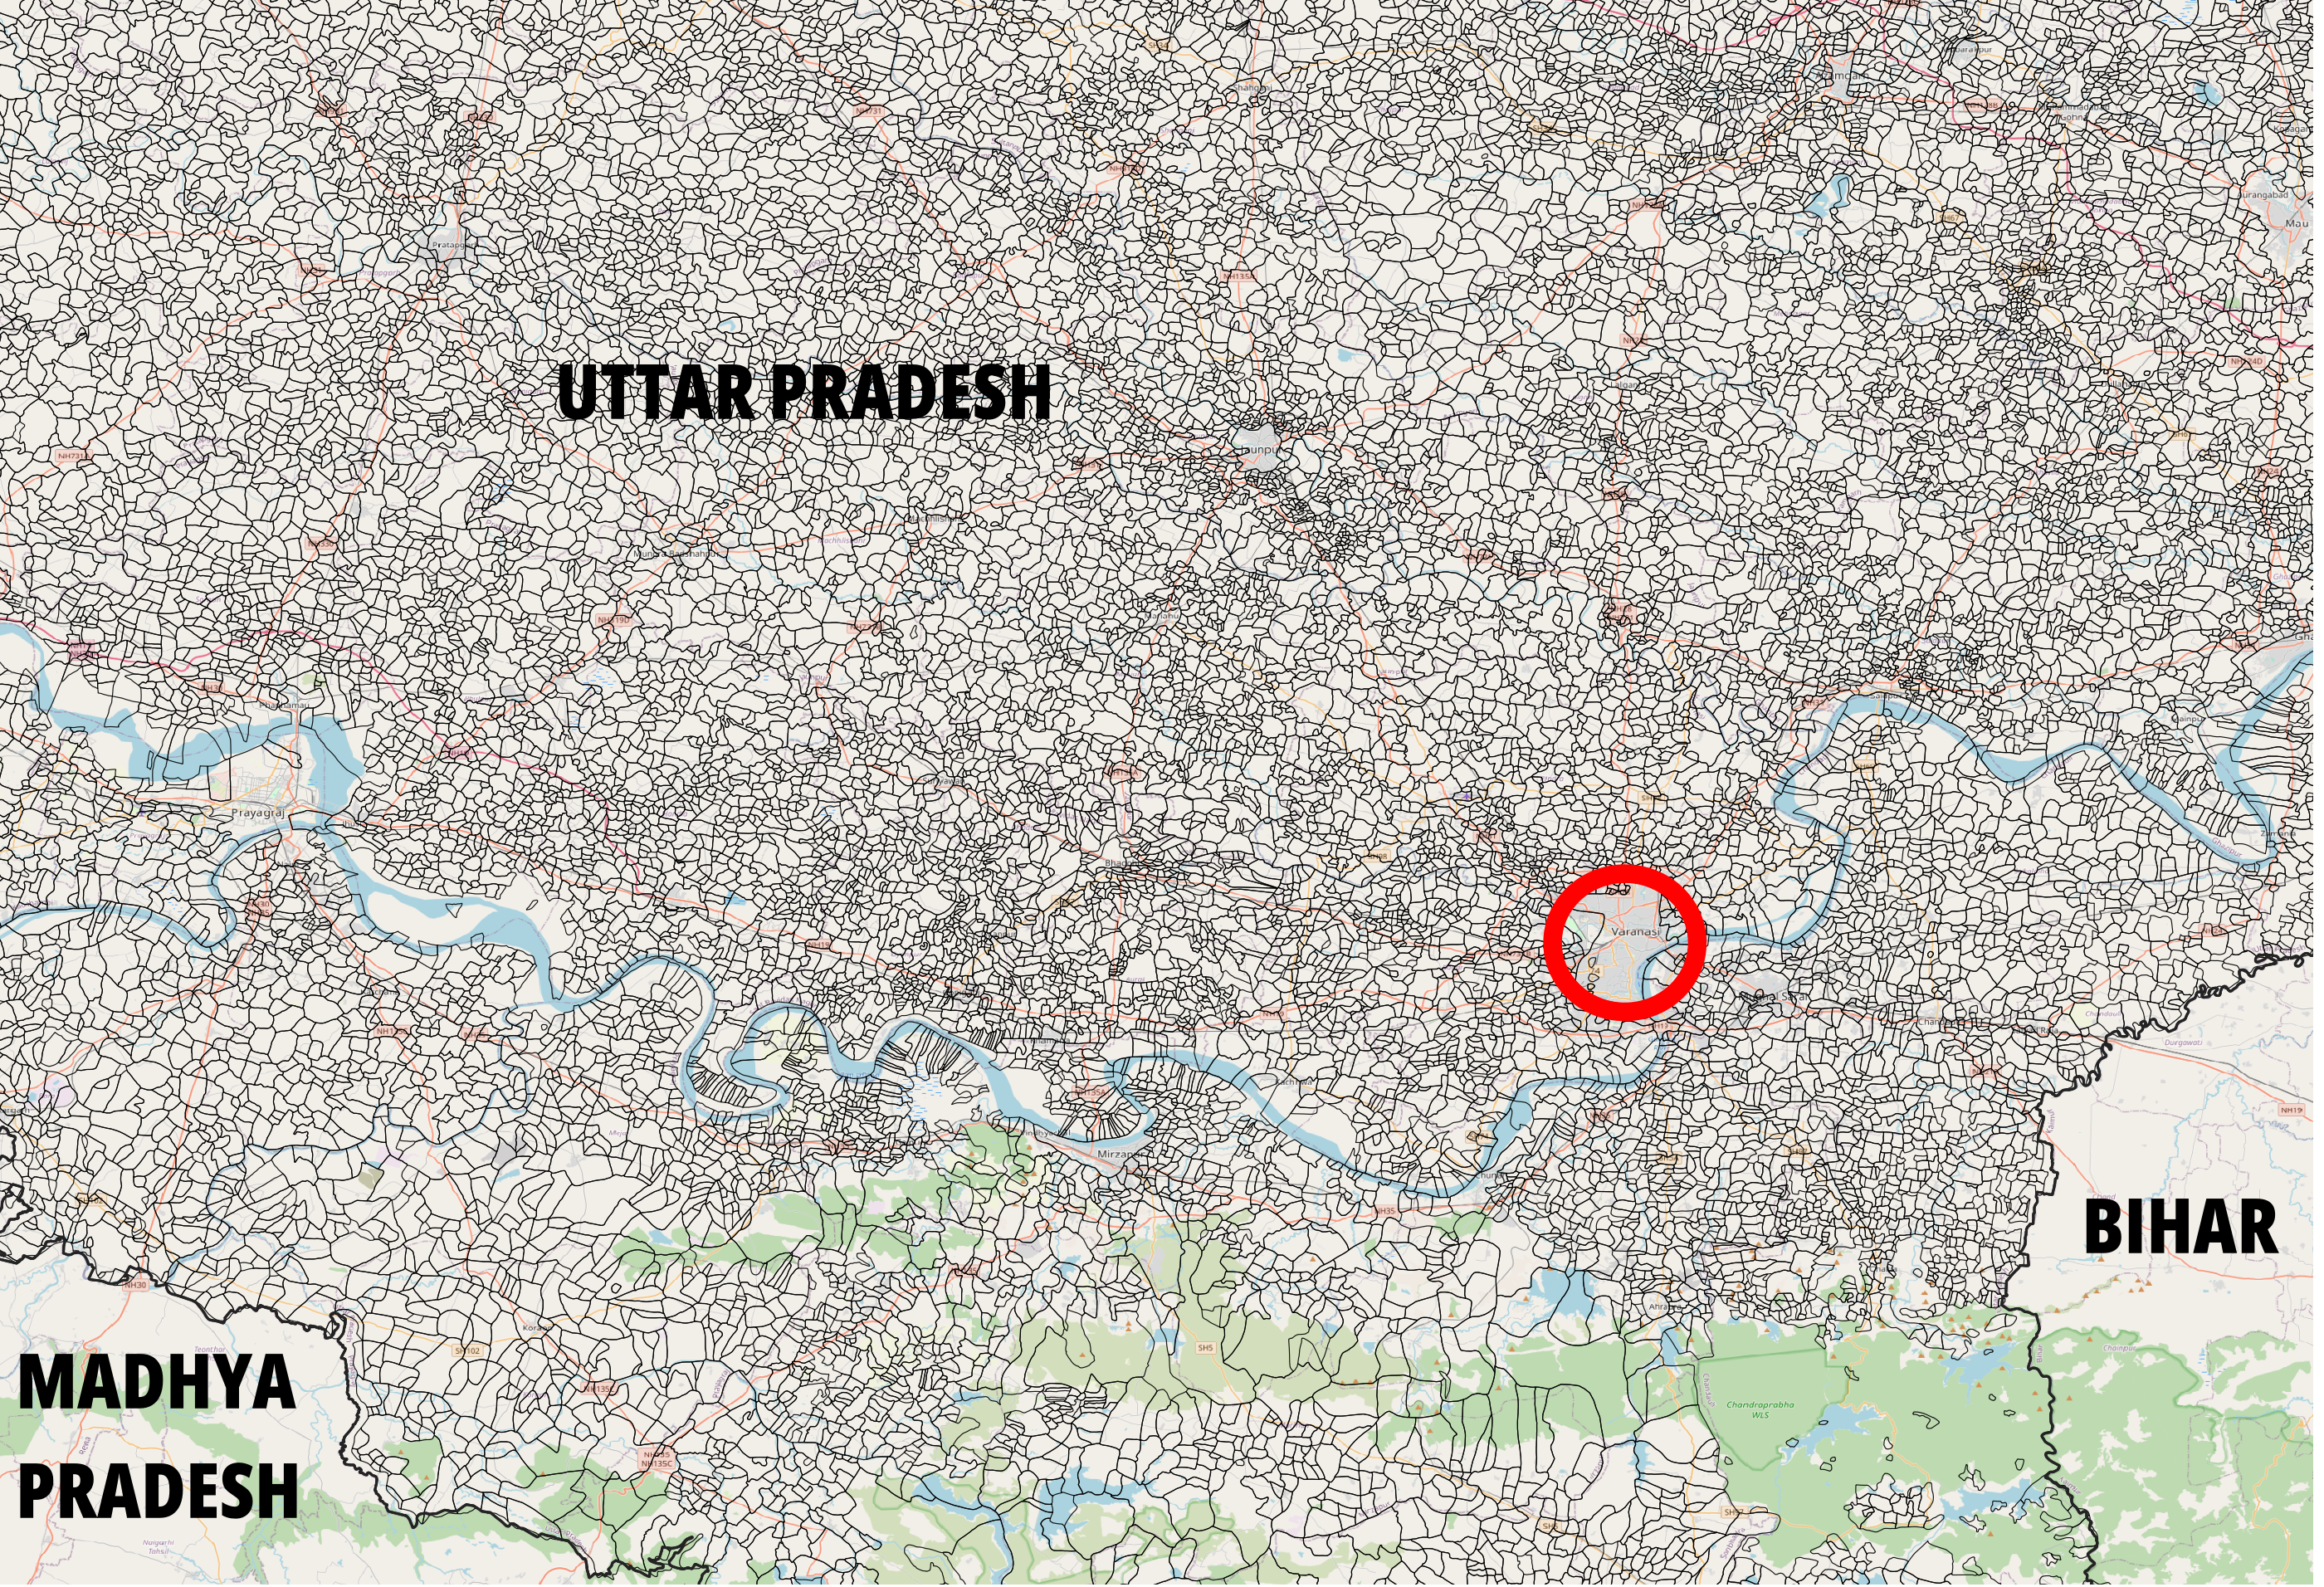
\includegraphics[width=0.9\textwidth]{images/shrid_desc.png}
                \caption{Red circle shows Varanasi.}
            \end{figure}
        \end{onlyenv}
    \end{frame}
    \begin{frame}{Economic Indicators}
        \textbf{Night lights}
        \begin{description}
            \item[Why?] Strong correlation with GDP growth even at subnational level \parencite{doll2006}.
            \item[Source] NASA, harmonized across satellites by \textcite{Li2020}, yearly data.
        \end{description}
        \pause
        \textbf{Built-up area}
        \begin{description}
            \item[Why?] Detects economic activity at highly local levels \parencite{baragwanath2021}.
            \item[Source] ESA, Copernicus GHSL product, five-year intervals.
        \end{description}
    \end{frame}
    
    \begin{frame}{Environmental Indicators}
    \begin{onlyenv}<1>
        \textbf{PM2.5 air quality}
        \begin{description}
            \item[Why?] Respected measure of environmental degradation \parencite{caviglia2009}.
            \item[Source] SHRUG v2, Development Data Lab cf.~\textcite{donkelaar2021}.
        \end{description}
        \pause{}
        \textbf{Land surface temperature}
        \begin{description}
            \item[Why?] Long-run changes from environmental degradation, global warming \parencite{esa}.
            \item[Source] NASA MODIS, yearly aggregates from 8-weekly data.
        \end{description}
    \end{onlyenv}
    \begin{onlyenv}<2>
        \textbf{PM2.5 air quality}
        \begin{description}
            \item[Why?] Respected measure of environmental degradation \parencite{caviglia2009}.
            \item[Source] SHRUG v2, Development Data Lab cf.~\textcite{donkelaar2021}.
        \end{description}
        \textbf{Land surface temperature}
        \begin{description}
            \item[Why?] Long-run changes from environmental degradation, global warming \parencite{esa}.
            \item[Source] NASA MODIS, yearly aggregates from 8-weekly data.
        \end{description}
    \end{onlyenv}
    \begin{onlyenv}<3>
        \textbf{Forest cover}
        \begin{description}
            \item[Why?] Relevant for infra growth, also used for horizontal devolution \parencite{wang2003,finance2020}.
            \item[Source] SHRUG v2, Development Data Lab, Terra MODIS (NASA).
        \end{description}
    \end{onlyenv}
    \end{frame}

    \begin{frame}[standout]
        \begin{figure}
            \centering
            \includegraphics[width=\textwidth]{images/ntl_hp.png}
        \end{figure}
    \end{frame}

    \section{Model and Findings}
    \begin{frame}{General Quadratic Model}
        \begin{equation*}
            \text{Env}_{it} = \beta_0 + \beta_1(\text{Econ}_{it}) + \beta_1(\text{Econ}_{it}^2) + \eta_i + \gamma_t + \epsilon_{it} 
            % \text{Env}_{it} = \beta_0 + \beta_1(\text{Econ}_{it}) + \beta_1(\text{Econ}_{it}^2) + \eta_i + \epsilon_{it} 
        \end{equation*}\\[1em]
        where:
        \begin{itemize}
            \item $\text{Env}_{it}$ $=$ environmental index value at area $i$ at time $t$.
            \item $\text{Econ}_{it}$ $=$ economic index value at area $i$ at time $t$.
            \item $\eta_i$ $=$ \textit{shrid}-level fixed effects.
            \item $\gamma_i$ $=$ year fixed effects.
            \item $\epsilon_{it}$ $=$ idiosyncratic error term.
        \end{itemize}
    \end{frame}

    \begin{frame}{Model 1: Night Lights}
        \begin{onlyenv}<1>
            
% Table created by stargazer v.5.2.3 by Marek Hlavac, Social Policy Institute. E-mail: marek.hlavac at gmail.com
% Date and time: Mon, Mar 03, 2025 - 02:14:27
\begin{table}[!htbp] \centering 
\begin{tabular}{@{\extracolsep{5pt}}lccc} 
\\[-2.4ex]\hline 
\hline \\[-2.4ex] 
 & \multicolumn{3}{c}{\textit{Dependent variable:}} \\ 
\cline{2-4} 
\\[-2.4ex] & \multicolumn{3}{c}{Environmental Index$_{VCF,PM25}$} \\ 
\\[-2.4ex] & (1) & (2) & (3)\\ 
\hline \\[-2.4ex] 
 NightLights & $-$0.025$^{***}$ & $-$0.018$^{***}$ & 0.270$^{***}$ \\ 
  & (0.001) & (0.001) & (0.001) \\ 
  & & & \\ 
 NightLights$^2$ & 0.022$^{***}$ & 0.016$^{***}$ & 0.003$^{***}$ \\ 
  & (0.0003) & (0.0002) & (0.0003) \\ 
  & & & \\ 
\hline \\[-2.4ex] 
PCA & Yes & No & No \\ 
TWFE & Yes & Yes & No \\ 
\hline 
\hline \\[-2.4ex] 
\textit{Note:}  & \multicolumn{3}{r}{$^{*}$p$<$0.1; $^{**}$p$<$0.05; $^{***}$p$<$0.01} \\ 
\end{tabular} 
\end{table} 

        \end{onlyenv}
        \begin{onlyenv}<2>
            \begin{figure}
                \centering
                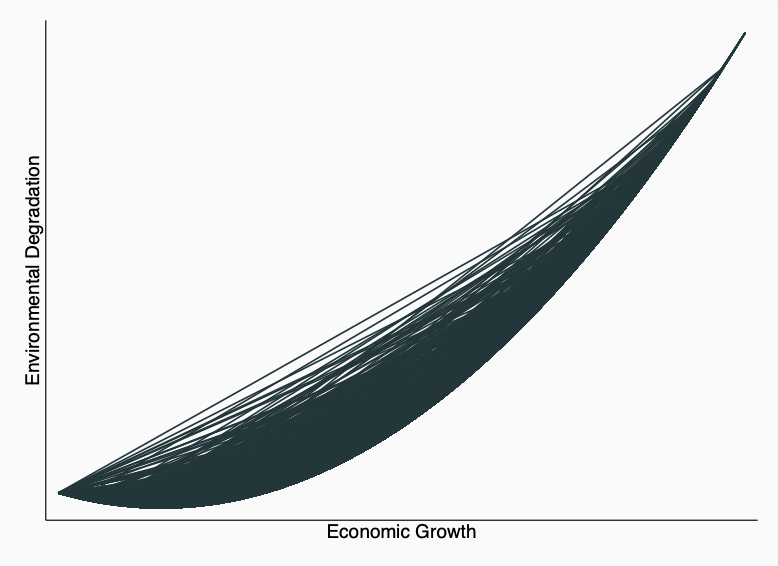
\includegraphics[width=0.8\textwidth]{images/presentation/model1.png}
            \end{figure}
        \end{onlyenv}
    \end{frame} % add graph

    \begin{frame}{Model 2: Adding Built-up Area} % change 2 for econst
        \begin{onlyenv}<1>
            
% Table created by stargazer v.5.2.3 by Marek Hlavac, Social Policy Institute. E-mail: marek.hlavac at gmail.com
% Date and time: Mon, Mar 03, 2025 - 02:27:36
\begin{table}[!htbp] \centering 
\begin{tabular}{@{\extracolsep{5pt}}lccc} 
\\[-2.4ex]\hline 
\hline \\[-2.4ex] 
 & \multicolumn{3}{c}{\textit{Dependent variable:}} \\ 
\cline{2-4} 
\\[-2.4ex] & \multicolumn{3}{c}{Environmental Index$_{VCF,PM25}$} \\ 
\\[-2.4ex] & (1) & (2) & (3)\\ 
\hline \\[-2.4ex] 
 EconIndex & $-$0.061$^{***}$ & $-$0.061$^{***}$ & 0.002$^{***}$ \\ 
  & (0.003) & (0.00004) & (0.00003) \\ 
  & & & \\ 
 EconIndex$^2$ & 0.013$^{***}$ & 0.019$^{***}$ & 0.003$^{***}$ \\ 
  & (0.0004) & (0.0003) & (0.0003) \\ 
  & & & \\ 
\hline \\[-2.4ex] 
PCA & Yes & No & No \\ 
TWFE & Yes & Yes & No \\ 
\hline 
\hline \\[-2.4ex] 
\textit{Note:}  & \multicolumn{3}{r}{$^{*}$p$<$0.1; $^{**}$p$<$0.05; $^{***}$p$<$0.01} \\ 
\end{tabular} 
\end{table} 

        \end{onlyenv}
        \begin{onlyenv}<2>
            \begin{figure}
                \centering
                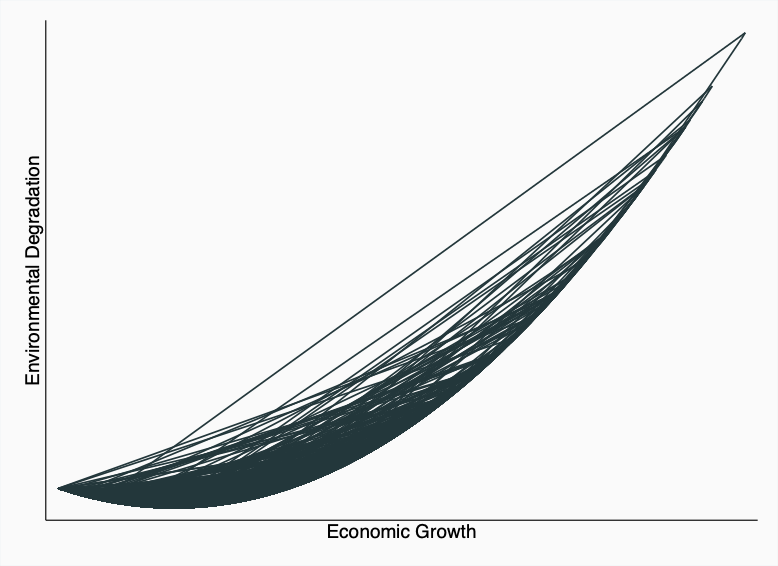
\includegraphics[width=0.8\textwidth]{images/presentation/model2.png}
            \end{figure}
        \end{onlyenv}
    \end{frame} % add graph

    \begin{frame}{Model 3: Adding Land Surface Temperature}
        \begin{onlyenv}<1>
            
% Table created by stargazer v.5.2.3 by Marek Hlavac, Social Policy Institute. E-mail: marek.hlavac at gmail.com
% Date and time: Mon, Mar 03, 2025 - 02:33:17
\begin{table}[!htbp] \centering 
\begin{tabular}{@{\extracolsep{5pt}}lccc} 
\\[-2.4ex]\hline 
\hline \\[-2.4ex] 
 & \multicolumn{3}{c}{\textit{Dependent variable:}} \\ 
\cline{2-4} 
\\[-2.4ex] & \multicolumn{3}{c}{Environmental Index$_{full}$} \\ 
\\[-2.4ex] & (1) & (2) & (3)\\ 
\hline \\[-2.4ex] 
 EconIndex & 0.038$^{***}$ & $-$0.061$^{***}$ & 0.414$^{***}$ \\ 
  & (0.003) & (0.003) & (0.003) \\ 
  & & & \\ 
 EconIndex$^2$ & 0.010$^{***}$ & 0.019$^{***}$ & $-$0.022$^{***}$ \\ 
  & (0.0004) & (0.0005) & (0.001) \\ 
  & & & \\ 
\hline \\[-2.4ex] 
PCA & Yes & No & No \\ 
TWFE & Yes & Yes & No \\ 
\hline 
\hline \\[-2.4ex] 
\textit{Note:}  & \multicolumn{3}{r}{$^{*}$p$<$0.1; $^{**}$p$<$0.05; $^{***}$p$<$0.01} \\ 
\end{tabular} 
\end{table} 

        \end{onlyenv}
        \begin{onlyenv}<2>
            \begin{figure}
                \centering
                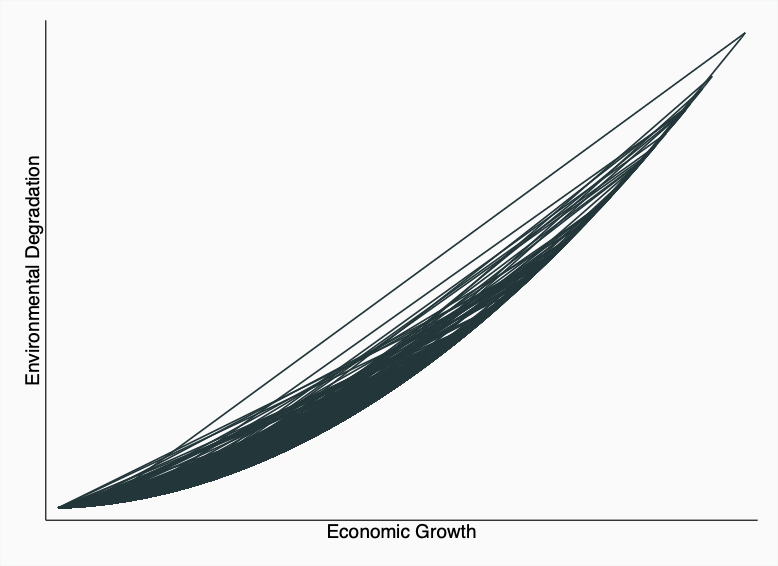
\includegraphics[width=0.8\textwidth]{images/presentation/model3.png}
            \end{figure}
        \end{onlyenv}
    \end{frame} % add graph


    % \begin{frame}{Model 4: Between Epochs}
    %     
% Table created by stargazer v.5.2.3 by Marek Hlavac, Social Policy Institute. E-mail: marek.hlavac at gmail.com
% Date and time: Mon, Mar 03, 2025 - 02:14:27
\begin{table}[!htbp] \centering 
\begin{tabular}{@{\extracolsep{5pt}}lccc} 
\\[-2.4ex]\hline 
\hline \\[-2.4ex] 
 & \multicolumn{3}{c}{\textit{Dependent variable:}} \\ 
\cline{2-4} 
\\[-2.4ex] & \multicolumn{3}{c}{Environmental Index$_{VCF,PM25}$} \\ 
\\[-2.4ex] & (1) & (2) & (3)\\ 
\hline \\[-2.4ex] 
 NightLights & $-$0.025$^{***}$ & $-$0.018$^{***}$ & 0.270$^{***}$ \\ 
  & (0.001) & (0.001) & (0.001) \\ 
  & & & \\ 
 NightLights$^2$ & 0.022$^{***}$ & 0.016$^{***}$ & 0.003$^{***}$ \\ 
  & (0.0003) & (0.0002) & (0.0003) \\ 
  & & & \\ 
\hline \\[-2.4ex] 
PCA & Yes & No & No \\ 
TWFE & Yes & Yes & No \\ 
\hline 
\hline \\[-2.4ex] 
\textit{Note:}  & \multicolumn{3}{r}{$^{*}$p$<$0.1; $^{**}$p$<$0.05; $^{***}$p$<$0.01} \\ 
\end{tabular} 
\end{table} 

    % \end{frame}

    % \begin{frame}{Introduction}
    %     \begin{itemize}
    %         \item Investigates the trade-off between economic growth and environmental sustainability.
    %         \item Uses high-resolution geospatial data for Himachal Pradesh and Uttarakhand.
    %         \item Develops a novel dataset of economic and environmental indicators over two decades.
    %     \end{itemize}
    % \end{frame}
    
    % \begin{frame}{Context: Why Build Infrastructure?}
    %     \begin{itemize}
    %         \item Economic, political, and administrative motivations.
    %         \item Border security concerns with China, Nepal, and Bhutan.
    %         \item Economic transition from agriculture to manufacturing and services.
    %         \item Role of infrastructure in connectivity, digital access, and energy generation.
    %     \end{itemize}
    % \end{frame}
    
    % \begin{frame}{Theoretical Framework: Environmental Kuznets Curve (EKC)}
    %     \begin{itemize}
    %         \item Hypothesis: Inverted-U relationship between economic growth and environmental degradation.
    %         \item Early stages: Growth leads to increased degradation.
    %         \item Later stages: Growth enables sustainability efforts.
    %         \item Contradictory findings in recent literature.
    %     \end{itemize}
    % \end{frame}
    
    % \begin{frame}{Data}
    %     \begin{itemize}
    %         \item Study unit: SHRUG village/town-level data.
    %         \item Economic indicators: Night-time lights, built-up area.
    %         \item Environmental indicators: Air quality (PM2.5), forest cover, land surface temperature.
    %         \item Data sources: NASA MODIS, GHSL, VIIRS, DMSP-OLS.
    %     \end{itemize}
    % \end{frame}
    
    % \begin{frame}{Findings: Temporal Shifts in Himachal Pradesh}
    %     \begin{itemize}
    %         \item Early 2000s - Mid 2000s: Forest cover increases in northern districts, declines in southern regions.
    %         \item 2010s: Growth in night-time lights, economic activity expands.
    %     \end{itemize}
    % \end{frame}
    
    % \begin{frame}{Findings: Temporal Shifts in Uttarakhand}
    %     \begin{itemize}
    %         \item Early 2000s - Mid 2000s: Forest cover increases in the north, declines in the south.
    %         \item Mid 2000s - 2010s: Widespread forest cover loss.
    %         \item Post-2010: Recovery in forest cover.
    %         \item Night-time lights show growth across all periods.
    %     \end{itemize}
    % \end{frame}
    
    % \begin{frame}{Model Specification}
    %     \begin{itemize}
    %         \item Quadratic fixed-effects model:
    %         \item Economic Index (NTL, built-up area) vs. Environmental Index (PM2.5, forest cover, LST).
    %         \item Fixed effects used based on Hausman test.
    %     \end{itemize}
    % \end{frame}
    
    % \begin{frame}{Regression Results: First Epoch}
    %     \begin{itemize}
    %         \item Estimated relationship follows the EKC (inverted U-shape).
    %         \item Economic growth initially leads to environmental degradation, then stabilizes.
    %     \end{itemize}
    % \end{frame}
    
    % \begin{frame}{Regression Results: Second Epoch}
    %     \begin{itemize}
    %         \item Relationship reverses to a U-shape.
    %         \item Economic growth initially reduces degradation but later exacerbates it.
    %     \end{itemize}
    % \end{frame}
    
    % \begin{frame}{Discussion}
    %     \begin{itemize}
    %         \item Results suggest heterogeneity across time.
    %         \item EKC not stable in ecologically sensitive regions.
    %         \item Potential tipping point in Himalayan environmental dynamics.
    %     \end{itemize}
    % \end{frame}
    
    \begin{frame}{Bottom Line}
        \begin{itemize}
            \item Economy-environment trade-offs in the Himalayas - an ecologically-sensitive region - are complex.
            \item EKC model fails when applied to localized contexts.
            \item Future research: pinpoint specific projects to build a treatment group for causal analysis, new estimation methods including GMM, causal machine learning.
        \end{itemize}
    \end{frame}

    \begin{frame}{Policy Implications}
        \begin{itemize}
            \item Centralized policy can have heterogenous outcomes.
            \item Need for localized, dynamic policy frameworks.
            \item Underlines the importance of ecological risk assessments.
            \item Emphasis on renewable energy, sustainable urban planning.
        \end{itemize}
    \end{frame}
    
    \begin{frame}[standout]
        Thank you.\\[2em]
        
        Our dataset is open-sourced at:

        github.com/RitwizSarma/himalayan-env\\[2em]

        Open to questions/comments.
    \end{frame}
    

\end{document}